\section{Eichung und Bestimmung der Wellenl�nge des Lasers}
In diesem Abschnitt soll das �bersetzungsverh�ltnis zwischen Schraube und Spiegel und die Wellenl�nge des Lasers bestimmt werden. Zuvor muss noch die x-Position in Lab-View und der Millimeterschraube geeicht werden.

\subsection{Eichung}
\label{Eichung}
Die x-Werte in Lab-View m�ssen den realen Positionen der Millimeterschraube zugeordnet werden. Bei der Bestimmung wird von einem linearem Zusammenhang ausgegangen. F�r die Eichung wird die Schraube gedreht, dabei wird in regelm��igen Abst�nden die Position im Interferogramm mit Lab-View aufgenommen. Der Fehler der Schraubenposition wird mit 0,5$\mu$m angenommen (eine halbe Skaleneinheit). F�r den Fit wurde Gleichung \ref{eqn:lin_fit} verwendet, A beschreibt dabei die Steigung und B das Offset. Der ist in Abbildung \ref{fig:eichung_laser} zu sehen. Aus dem Fit ergebe sich die Parameter in Tabelle \ref{tab:eichung_laser}.
\begin{align}
\label{eqn:lin_fit}
f(x) = A \cdot x + B
\end{align}

\begin{figure}[H]
\centering
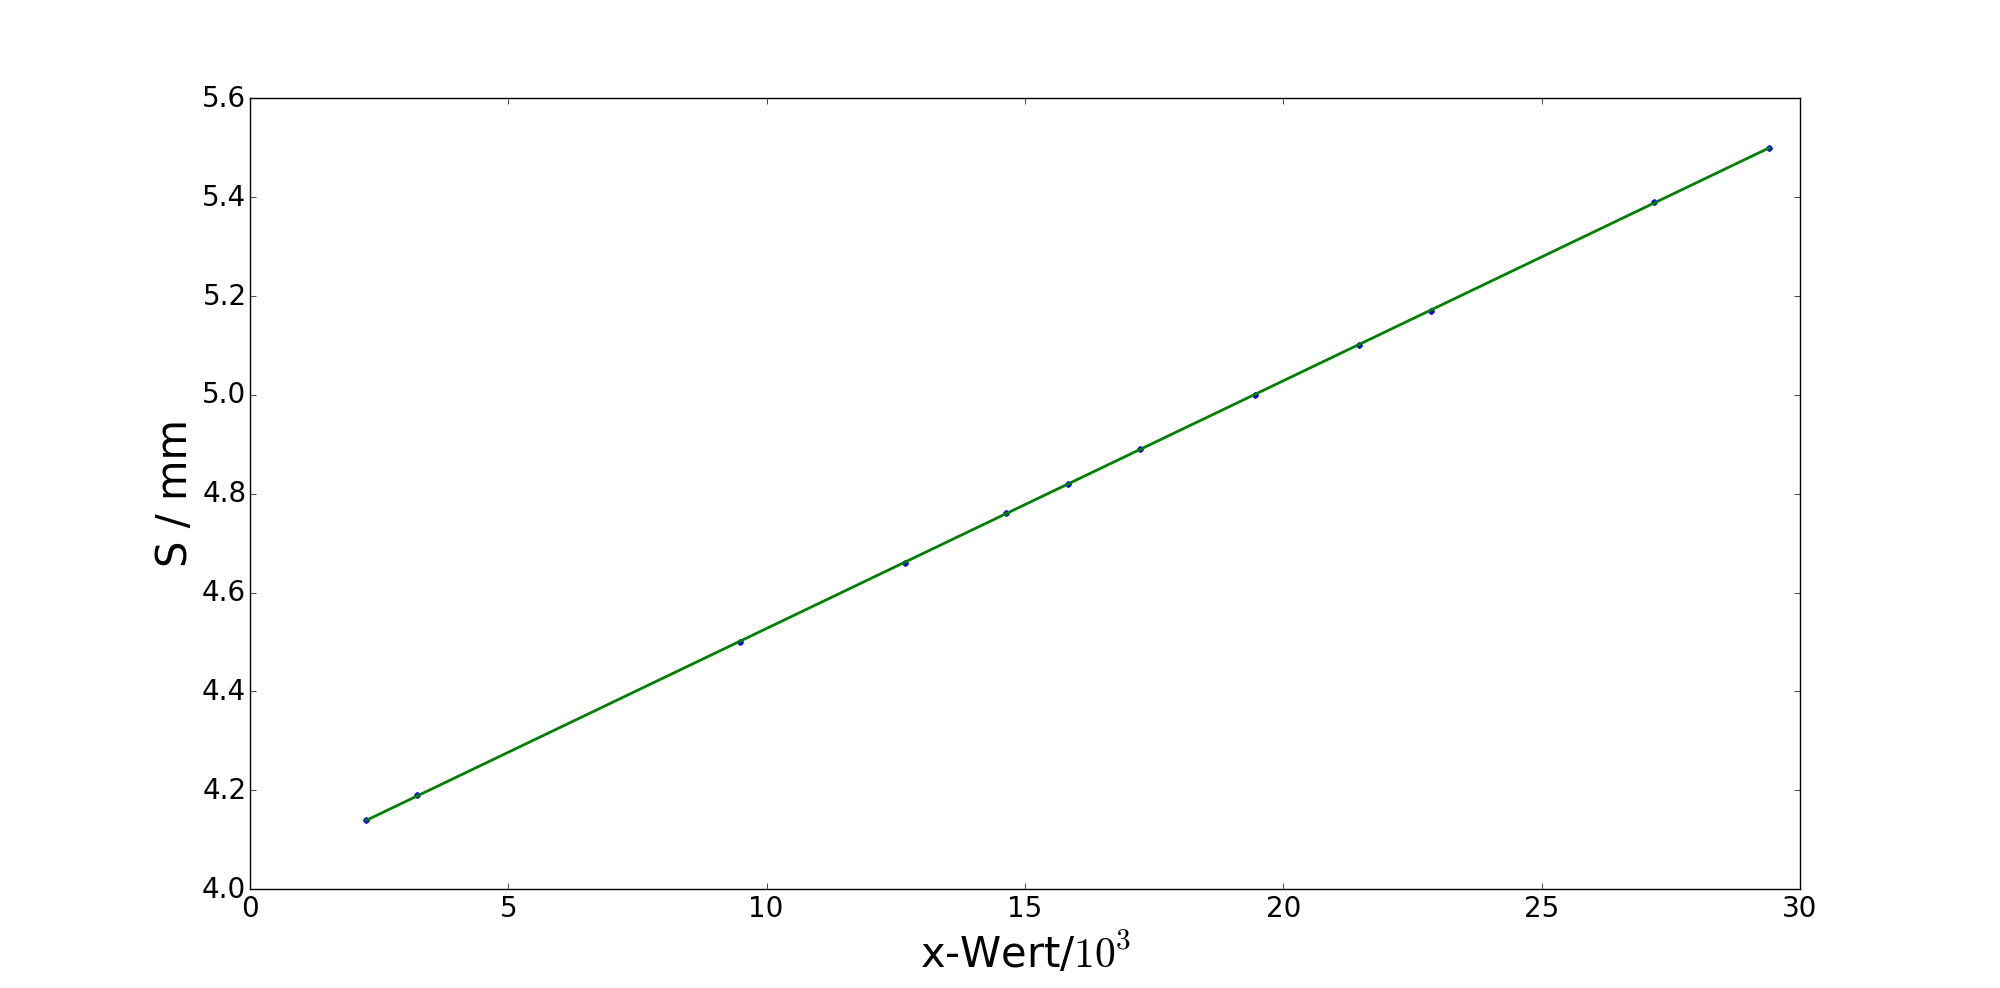
\includegraphics[scale = 0.33]{eichung_laser.png}
\caption{Linearer Fit f�r den Zusammenhang zwischen Kanal in Lab-View und der Position der Millimeterschraube. Die Fehler der Messpunkte sind so klein, dass sie nicht zu erkennen sind.}
\label{fig:eichung_laser}
\end{figure}

\begin{table}[H]
\centering
\caption{Parameter aus dem Fit f�r den Zusammenhang zwischen Kanal in Lab-View und der Position der Millimeterschraube}
\label{tab:eichung_laser}
\begin{tabular}{|c|c|}
\hline Parameter & Wert \\ 
\hline A / mm & 5.009(8)e-05 \\ 
\hline B / mm & 4.0263(9) \\ 
\hline $\chi_{red}^2$ & 0.78 \\ 
\hline 
\end{tabular} 
\end{table}

\subsection{Bestimmund der Wellenl�nge des Lasers}
Mit der zuvor durchgef�hrten Eichung kann nun die Wellenl�nge $\lambda$ des Lasers bestimmt werden. Die Wellenl�nge wird aus dem Gangunterschied s, der Anzahl der Interferenzmaxima n und dem �bersetzungsverh�ltnis k bestimmt. F�r das �bersetzungsverh�ltnis wird ein Wert von k=5 angenommen. Die Wellenl�nge ergibt sich nach Gleichung \ref{eqn:wellenlaenge}.

\begin{align}
\label{eqn:wellenlaenge}
\lambda = \frac{2s}{5n}
\end{align}

Das aufgenommen Interferogramm ist in Abbildung \ref{fig:laser} zu sehen.

\begin{figure}[H]
\centering
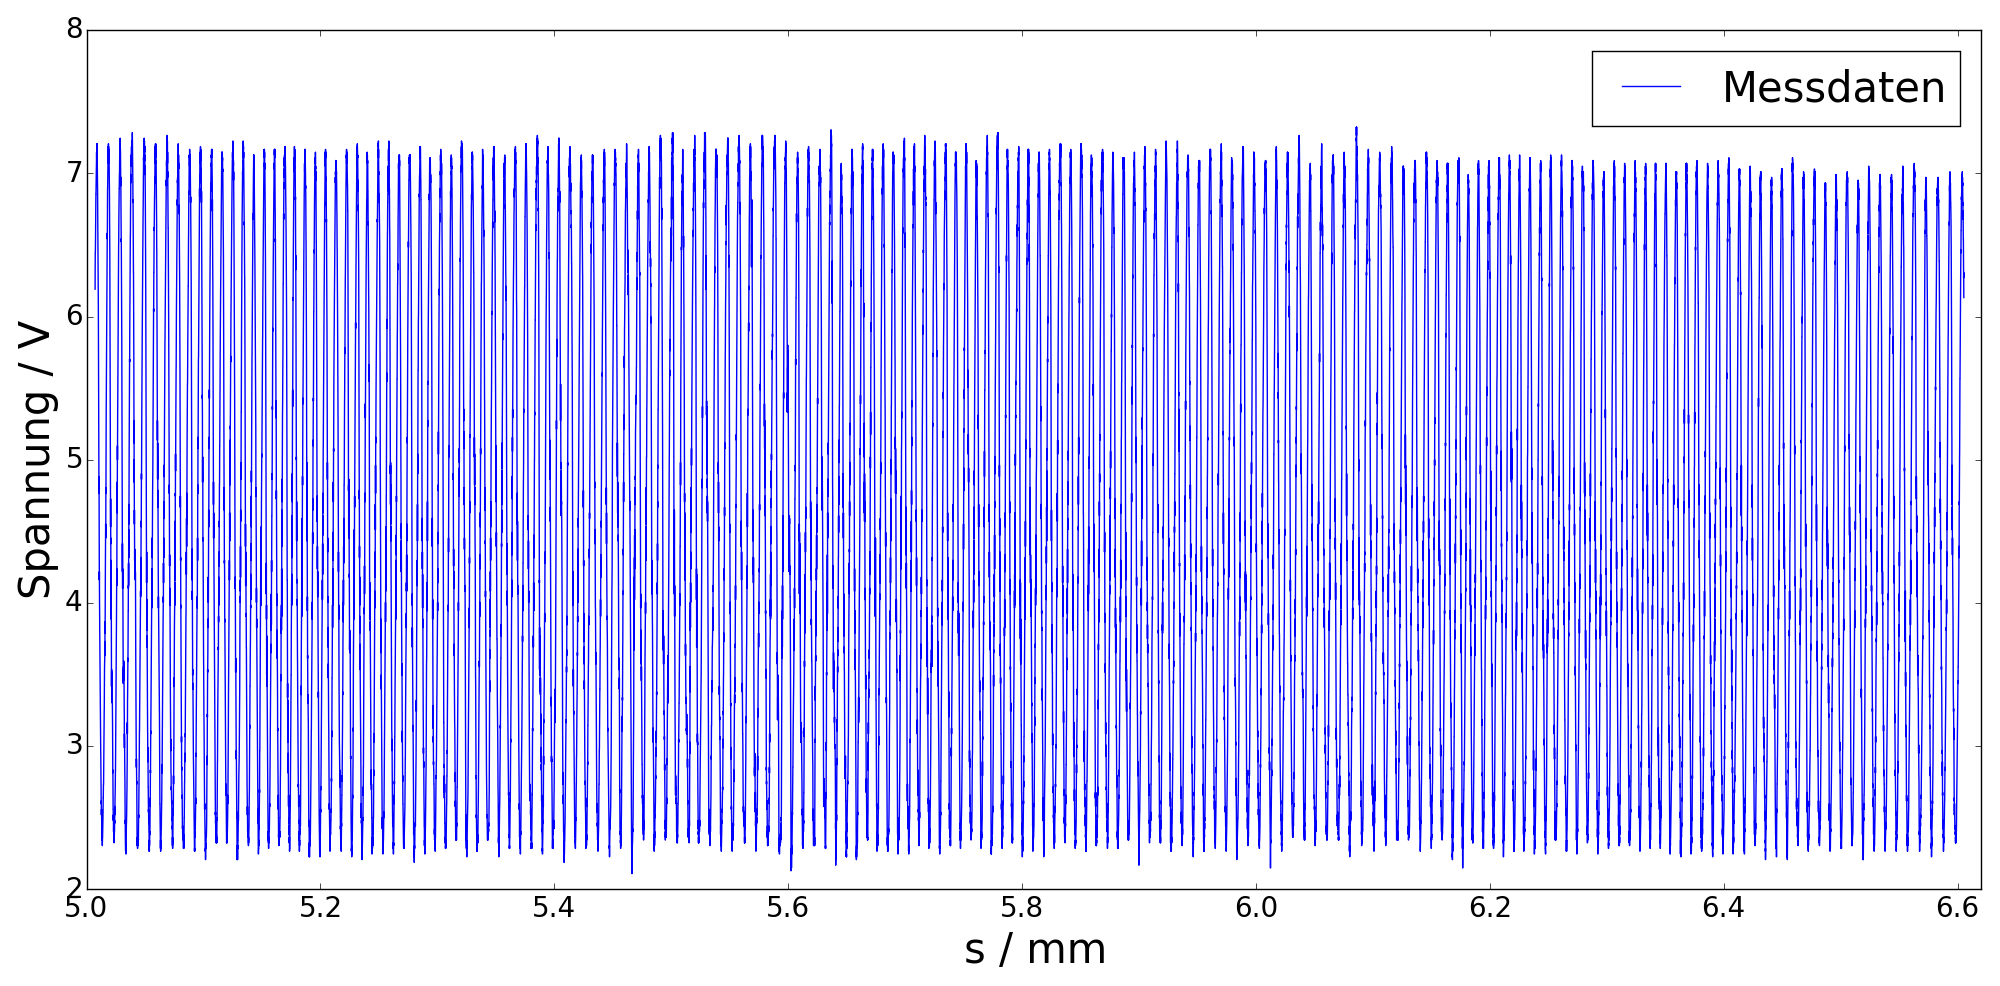
\includegraphics[scale = 0.33]{laser_interferogram.png}
\caption{Interferogramm des Lasers. Es wurden 173 Peaks aufgenommen}
\label{fig:laser}
\end{figure}

Mit der zuvor durchgef�hrten Eichung wird der Gangunterschied der x-Position in eine reelle Wegdifferenz umgerechnet, der Fehler ergibt sich nach Fehlerfortpflanzung auf die Geradengleichung. Die Anzahl der Maxima wurde als Fehlerlos angenommen. Die Messdaten sind in Tabelle \ref{tab:wellenlaenge} eingetragen. Aus den bestimmten Wellenl�ngen ergibt sich ein Mittelwert von 3.732(9) $\mu$m. 

\begin{table}
\centering
\caption{Messergebnisse f�r die Bestimmung der Wellenl�nge}
\label{tab:wellenlaenge}
\begin{tabular}{|c|c|c|c|c|}
\hline n & x$_1$ / mm & x$_2$ / mm & s / mm & $\lambda$ / $\mu$m \\ 
\hline 173 & 5.0088(3) & 6.6040(3) & 1.5952(4) & 3.688(9) \\ 
\hline 172 & 5.0107(3) & 6.6040(3) & 1.5933(4) & 3.705(9) \\ 
\hline 171 & 5.0127(3) & 6.6040(3) & 1.5913(4) & 3.722(9) \\ 
\hline 170 & 5.0151(3) & 6.6040(3) & 1.5889(4) & 3.738(9) \\ 
\hline 169 & 5.0493(3) & 6.6040(3) & 1.5547(4) & 3.739(9) \\ 
\hline 168 & 5.0589(3) & 6.6040(3) & 1.5451(4) & 3.742(9) \\ 
\hline 167 & 5.0689(3) & 6.6040(3) & 1.5351(4) & 3.743(9) \\ 
\hline 166 & 5.0784(3) & 6.6040(3) & 1.5256(4) & 3.746(9) \\ 
\hline 165 & 5.0884(3) & 6.6040(3) & 1.5159(4) & 3.746(9) \\ 
\hline 164 & 5.0975(3) & 6.6040(3) & 1.5600(4) & 3.752(9) \\ 
\hline 
\end{tabular} 
\end{table}


Um ein besseres Ergebnis zu erhalten, wird das eigentliche �bersetzungsverh�ltnis $k_e$ mit Gleichung \ref{eqn:uebersetzungsverhaeltniss} bestimmt. Dabei wurde f�r $\lambda$ der Literaturwert von 3,39$\mu$m verwendet (vlg \ref{eqn:uebersetzungsverhaeltniss}). Der korrigierte �bersetzungsfaktor ergibt sich mit 5.42(1).

\begin{align}
\label{eqn:uebersetzungsverhaeltniss}
k_e = \frac{2s}{n\lambda}
\end{align}
